\begin{figure}[h]
    \centering



\tikzset{every picture/.style={line width=0.75pt}} %set default line width to 0.75pt        

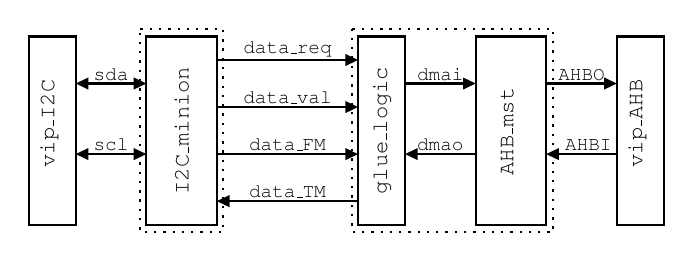
\begin{tikzpicture}[x=0.85pt,y=0.85pt,yscale=-1,xscale=1]
%uncomment if require: \path (0,300); %set diagram left start at 0, and has height of 300

%Shape: Rectangle [id:dp4079589054406878] 
\draw   (70,60) -- (100,60) -- (100,140) -- (70,140) -- cycle ;
%Shape: Rectangle [id:dp32174966169393304] 
\draw   (160,60) -- (180,60) -- (180,140) -- (160,140) -- cycle ;
%Shape: Rectangle [id:dp8708617087982464] 
\draw   (210,60) -- (240,60) -- (240,140) -- (210,140) -- cycle ;
%Shape: Rectangle [id:dp6411738601274033] 
\draw   (270,60) -- (290,60) -- (290,140) -- (270,140) -- cycle ;
%Shape: Rectangle [id:dp537675519060894] 
\draw   (20,60) -- (40,60) -- (40,140) -- (20,140) -- cycle ;
%Shape: Rectangle [id:dp738814812078364] 
\draw  [dash pattern={on 0.84pt off 2.51pt}] (67.5,56.75) -- (102.5,56.75) -- (102.5,143.25) -- (67.5,143.25) -- cycle ;
%Shape: Rectangle [id:dp16028896948499805] 
\draw  [dash pattern={on 0.84pt off 2.51pt}] (157.6,56.7) -- (243,56.7) -- (243,143.2) -- (157.6,143.2) -- cycle ;
%Straight Lines [id:da14064721488292253] 
\draw    (43,80) -- (67,80) ;
\draw [shift={(70,80)}, rotate = 180] [fill={rgb, 255:red, 0; green, 0; blue, 0 }  ][line width=0.08]  [draw opacity=0] (5.36,-2.57) -- (0,0) -- (5.36,2.57) -- cycle    ;
\draw [shift={(40,80)}, rotate = 0] [fill={rgb, 255:red, 0; green, 0; blue, 0 }  ][line width=0.08]  [draw opacity=0] (5.36,-2.57) -- (0,0) -- (5.36,2.57) -- cycle    ;
%Straight Lines [id:da4386174351987262] 
\draw    (43,110) -- (67,110) ;
\draw [shift={(70,110)}, rotate = 180] [fill={rgb, 255:red, 0; green, 0; blue, 0 }  ][line width=0.08]  [draw opacity=0] (5.36,-2.57) -- (0,0) -- (5.36,2.57) -- cycle    ;
\draw [shift={(40,110)}, rotate = 0] [fill={rgb, 255:red, 0; green, 0; blue, 0 }  ][line width=0.08]  [draw opacity=0] (5.36,-2.57) -- (0,0) -- (5.36,2.57) -- cycle    ;
%Straight Lines [id:da5336477753811442] 
\draw    (100,70) -- (157,70) ;
\draw [shift={(160,70)}, rotate = 180] [fill={rgb, 255:red, 0; green, 0; blue, 0 }  ][line width=0.08]  [draw opacity=0] (5.36,-2.57) -- (0,0) -- (5.36,2.57) -- cycle    ;
%Straight Lines [id:da5216454033214535] 
\draw    (100,90) -- (157,90) ;
\draw [shift={(160,90)}, rotate = 180] [fill={rgb, 255:red, 0; green, 0; blue, 0 }  ][line width=0.08]  [draw opacity=0] (5.36,-2.57) -- (0,0) -- (5.36,2.57) -- cycle    ;
%Straight Lines [id:da06972034582349096] 
\draw    (100,110) -- (157,110) ;
\draw [shift={(160,110)}, rotate = 180] [fill={rgb, 255:red, 0; green, 0; blue, 0 }  ][line width=0.08]  [draw opacity=0] (5.36,-2.57) -- (0,0) -- (5.36,2.57) -- cycle    ;
%Straight Lines [id:da16308212972517788] 
\draw    (103,130) -- (160,130) ;
\draw [shift={(100,130)}, rotate = 0] [fill={rgb, 255:red, 0; green, 0; blue, 0 }  ][line width=0.08]  [draw opacity=0] (5.36,-2.57) -- (0,0) -- (5.36,2.57) -- cycle    ;
%Straight Lines [id:da04498796035539643] 
\draw    (180,80) -- (207,80) ;
\draw [shift={(210,80)}, rotate = 180] [fill={rgb, 255:red, 0; green, 0; blue, 0 }  ][line width=0.08]  [draw opacity=0] (5.36,-2.57) -- (0,0) -- (5.36,2.57) -- cycle    ;
%Straight Lines [id:da9819499243578742] 
\draw    (183,110) -- (210,110) ;
\draw [shift={(180,110)}, rotate = 0] [fill={rgb, 255:red, 0; green, 0; blue, 0 }  ][line width=0.08]  [draw opacity=0] (5.36,-2.57) -- (0,0) -- (5.36,2.57) -- cycle    ;
%Straight Lines [id:da4892721330990073] 
\draw    (240,80) -- (267,80) ;
\draw [shift={(270,80)}, rotate = 180] [fill={rgb, 255:red, 0; green, 0; blue, 0 }  ][line width=0.08]  [draw opacity=0] (5.36,-2.57) -- (0,0) -- (5.36,2.57) -- cycle    ;
%Straight Lines [id:da9092580589886958] 
\draw    (243,110) -- (245.8,110) -- (270,110) ;
\draw [shift={(240,110)}, rotate = 0] [fill={rgb, 255:red, 0; green, 0; blue, 0 }  ][line width=0.08]  [draw opacity=0] (5.36,-2.57) -- (0,0) -- (5.36,2.57) -- cycle    ;

% Text Node
\draw (28.5,97) node  [font=\footnotesize,rotate=-270] [align=left] {{\fontfamily{pcr}\selectfont vip\_I2C}};
% Text Node
\draw (85,100) node  [font=\footnotesize,rotate=-270] [align=left] {{\fontfamily{pcr}\selectfont I2C\_minion}};
% Text Node
\draw (170,100) node  [font=\footnotesize,rotate=-270] [align=left] {{\fontfamily{pcr}\selectfont glue\_logic}};
% Text Node
\draw (223.4,100.4) node  [font=\footnotesize,rotate=-270] [align=left] {{\fontfamily{pcr}\selectfont AHB\_mst}};
% Text Node
\draw (278.5,97) node  [font=\footnotesize,rotate=-270] [align=left] {{\fontfamily{pcr}\selectfont vip\_AHB}};
% Text Node
\draw (55,80) node [anchor=south] [inner sep=0.75pt]  [font=\scriptsize] [align=left] {{\fontfamily{pcr}\selectfont sda}};
% Text Node
\draw (55,110) node [anchor=south] [inner sep=0.75pt]  [font=\scriptsize] [align=left] {{\fontfamily{pcr}\selectfont scl}};
% Text Node
\draw (130,70) node [anchor=south] [inner sep=0.75pt]  [font=\scriptsize] [align=left] {{\fontfamily{pcr}\selectfont data\_req}};
% Text Node
\draw (130,90) node [anchor=south] [inner sep=0.75pt]  [font=\scriptsize] [align=left] {{\fontfamily{pcr}\selectfont data\_val}};
% Text Node
\draw (130,110) node [anchor=south] [inner sep=0.75pt]  [font=\scriptsize] [align=left] {{\fontfamily{pcr}\selectfont data\_FM}};
% Text Node
\draw (130,130) node [anchor=south] [inner sep=0.75pt]  [font=\scriptsize] [align=left] {{\fontfamily{pcr}\selectfont data\_TM}};
% Text Node
\draw (195,80) node [anchor=south] [inner sep=0.75pt]  [font=\scriptsize] [align=left] {{\fontfamily{pcr}\selectfont dmai}};
% Text Node
\draw (195,110) node [anchor=south] [inner sep=0.75pt]  [font=\scriptsize] [align=left] {{\fontfamily{pcr}\selectfont dmao}};
% Text Node
\draw (255,80) node [anchor=south] [inner sep=0.75pt]  [font=\scriptsize] [align=left] {{\fontfamily{pcr}\selectfont AHBO}};
% Text Node
\draw (257.9,110) node [anchor=south] [inner sep=0.75pt]  [font=\scriptsize] [align=left] {{\fontfamily{pcr}\selectfont AHBI}};


\end{tikzpicture}
    \caption{I2C to AHB System Block Diagram}
    \label{fig:complete_system}
\end{figure}
